\documentclass[c_worksheet.tex]{subfiles}

\begin{document}
  
\chapter{Profiaufgaben}

\section{Linked List}

Eine Linked List ist eine Datenstruktur um viele Elemente in einer Liste zu speichern. Dabei merkt sich jedes Element der Liste wo sein Nachfolger zu finden ist. Die Elemente liegen also nicht wie bei einem Array hintereinander, sondern können überall im Speicher verteilt sein. \\

Erstelle als erstes eine Struktur um ein Listenelement zu speichern. Jedes Element soll sich einen Integer und die Adresse des Nachfolgers speichern. \\
Schreibe als nächstes eine Struktur ``Liste'', die sich ihre aktuelle Größe und die Adresse des ersten Listenelemts speichert.

\begin{figure}[h]
\centering
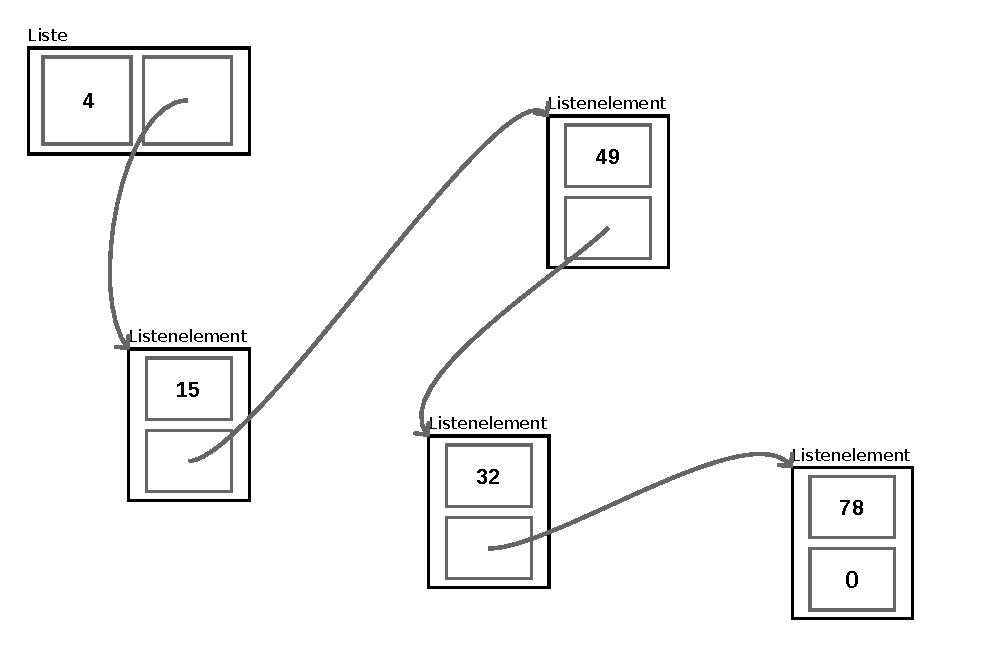
\includegraphics[width=0.8\textwidth]{./Grafiken/Aufgaben/linkedList}
\caption{Die Liste hat 4 Elemente [15,49,32,78]} 
\end{figure}

Die Speicheradresse 0 hat eine besondere Bedeutung. Wenn ein Pointer zur Adresse 0 zeigt, dann ist er kein valider Pointer, sondern signalisiert, dass er nicht auf ein Objekt zeigt. Die Adresse 0 darf außerdem nicht dereferenziert werden. Hier können wir das nutzen um das Ende der Liste zu bestimmen.\\

\begin{itemize}
  \item Schreibe eine Funktion die eine neue Liste ohne Elemente erstellt. Achte darauf die Größe und den Pointer auf das erste Elelemt richtig zu initialisieren.
  \item Schreibe zwei Funktionen um neue Elemente einzufügen. Eine um ein Elelemt hinten anhängt und eine um ein Elelemt vorne anzuhängen.
  \item Füge ein paar Elelemte in eine Liste ein und gib den Inhalt auf die Konsole aus. ``\textit{[1,3,8,...]}''
  \item Schreibe zwei Funktionen um Elemente aus der Liste zu löschen. Eine um das erste und eine um das letzte Element zu löschen.
  \item Schreibe eine Funktion ``contains'' die überprüft ob ein gegebener Integer in der Liste enthalten ist.
\end{itemize}

\textbf{Zusatzaufgabe:}\\
Erstelle eine Double Linked List, bei der jedes Elelemt die Adresse des Nachfolgers und des Vorgängers speichert. Diese soll alles können, was auch die Linked List konnte. Einige Operationen sollten damit einfacher umzusetzen sein.

\section{Sortieren von Arrays}

Hier geht es darum die Elemente in einem Array ihrer Größe nach zu sortieren. Wir benutzen ersteinmal nur Integer, weil wir diese schon mit \textbf{<}, \textbf{>}, \textbf{==}, \textbf{<=} und \textbf{>=} vergleichen können.

\subsection{Insertion Sort}
Angenommen du hast bereits ein Array, das bis zu einem bestimmten Punkt mit Werten gefüllt und sortiert ist. Wie könnte man dann eine neue Zahl einfügren, sodass das Array immernoch sortiert ist? Überlege dir dazu an welche Stelle die neue Zahl gehört, und wie du an dieser Stelle Platz schaffen kannst.

\begin{figure}[h]
\centering
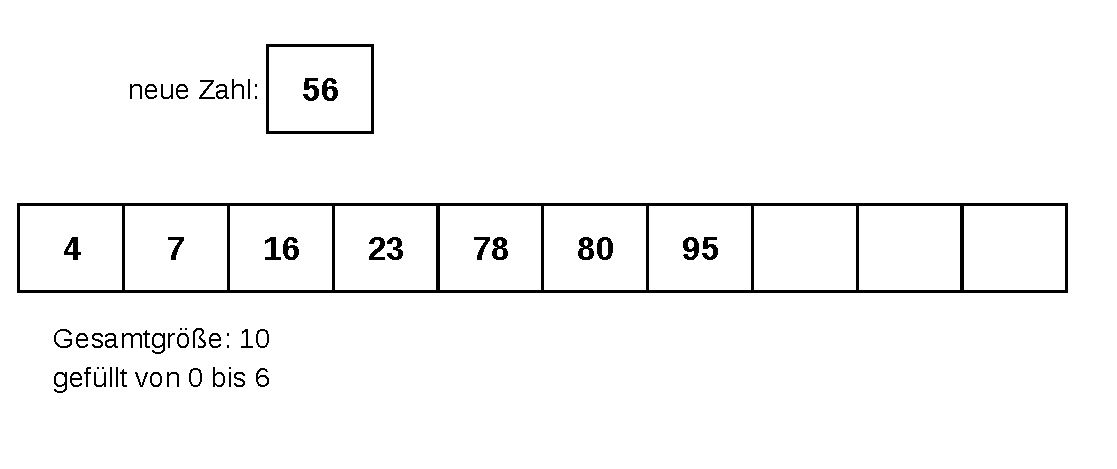
\includegraphics[width=0.7\textwidth]{./Grafiken/Aufgaben/insertionSort}
\caption{Ein sortiertes Array, in das ein neues Element eingefügt werden soll} 
\end{figure}

In einer vorherigen Aufgabe ging es darum das kleinste Element aus einem Array zu finden. Überlege dir nun wie du durch finden des kleinsten Elelemts und durch einfügen in eine sortierte Teilliste ein Array sortieren kannst.

\subsection{Bubble Sort}

Der Bubblesort Algorithmus schaut sich immer zwei benachbarte Elemente an und vertauscht diese gegebenenfalls. Überlege dir, welche Auswirkungen es hat damit einmal über das ganze Array zu laufen.

\begin{itemize}
  \item Schreibe eine Funktion die einmal über ein Array läuft und dabei immer zwei benachbarte Elemente miteinander vergleicht. Wenn die beiden Elemente falsch herum stehen, sollen sie vertauscht werden.
  \item Benutze die erste Funktion um ein Array zu sortieren. (Überlege dir wie oft die erste Funktion aufgerufen werden muss)
  \item Bubblesort lässt sich auch auf Double Linked Lists anwenden. Schreibe eine Funktion die eine Double Linked List sortiert.
\end{itemize}

\section{Blocksatz}

Die Aufgabe ist es eine lange Zeichenkette in Blocksatz auf der Konsole auszugeben. Das heißt jede Zeile soll gleich breit sein. Schreibe als erstes eine Funktion, die einen gegebenen Text in Zeilen aufspaltet. Der Text darf nur bei Leerzeichen auseinander gerissen werden um Zeilen zu bilden. Eine Zeile darf maximal so lang sein, wie die vorher festgelegte Textbreite. Viele Zeilen werden danach zu kurz sein. Schreibe eine Funktion, die eine Zeile nimmt und sie duch einfügen von Leerzeichen auf die richtige Länge bringt. Danach kann der Text Zeile für Zeile ausgegeben werden.\\

Normalerweise würde man den Text erst aus einer Datei einlesen. Hier gehen wir davon aus, dass er wie folgt gegeben ist:
\begin{lstlisting}[numbers=none]
char *inputText = "Ich bin ein Text. Und ich bin viel zu " \
        "lang um an einem Stueck auf der Konsole ausgegeben" \
        " zu werden. Fuer die Uebung sollte man mich " \
        "duch einen noch laengeren Text aus dem Internet" \
        " ersetzen.";
\end{lstlisting}
Das ist ein einziger String, der durch eine Null beendet wird.


\end{document}